% docs/slides/preamble.tex -- 五份 deck 共享
\documentclass[aspectratio=169,11pt]{beamer}

% ==== 中文与字体 ====
\usepackage[UTF8,fontset=none]{ctex}
\usepackage{fontspec}

\IfFontExistsTF{PingFang SC}{%
  \setCJKmainfont{PingFang SC}[BoldFont=PingFang SC,ItalicFont=PingFang SC,AutoFakeSlant=0.15]
  \setCJKsansfont{PingFang SC}[ItalicFont=PingFang SC,AutoFakeSlant=0.15]
  \setCJKmonofont{PingFang SC}
}{%
  \IfFontExistsTF{Source Han Sans SC}{%
    \setCJKmainfont{Source Han Sans SC}
    \setCJKsansfont{Source Han Sans SC}
  }{%
    \IfFontExistsTF{Noto Sans CJK SC}{%
      \setCJKmainfont{Noto Sans CJK SC}
      \setCJKsansfont{Noto Sans CJK SC}
    }{%
      \setCJKmainfont{Heiti SC}
      \setCJKsansfont{Heiti SC}
    }
  }
}

\IfFontExistsTF{Helvetica Neue}{\setmainfont{Helvetica Neue}}{%
  \IfFontExistsTF{Inter}{\setmainfont{Inter}}{}}
\IfFontExistsTF{JetBrains Mono}{\setmonofont{JetBrains Mono}[Scale=0.85]}%
  {\setmonofont{Menlo}[Scale=0.85]}

% ==== 颜色 ====
\usepackage{xcolor}
\definecolor{cMain}{HTML}{1F4E79}
\definecolor{cAccent}{HTML}{E07A1F}
\definecolor{cGray}{HTML}{595959}
\definecolor{cMute}{HTML}{F4F4F4}
\definecolor{cOK}{HTML}{2E7D32}
\definecolor{cBad}{HTML}{B23A3A}
\definecolor{cWarn}{HTML}{C8A300}

% ==== 主题 ====
\usepackage{tcolorbox}
\usetheme{metropolis}
\metroset{progressbar=frametitle,numbering=fraction,block=fill}
\setbeamercolor{frametitle}{bg=cMain,fg=white}
\setbeamercolor{progress bar}{fg=cAccent,bg=cMute}
\setbeamercolor{alerted text}{fg=cAccent}
\setbeamercolor{title}{fg=cMain}

% metropolis 默认尝试 Fira Sans，未安装时 fallback 到 Latin Modern Sans。
% 这里在主题加载后显式覆盖，强制使用 macOS 上一定存在的 Helvetica Neue，
% 跟中文 PingFang 风格一致；找不到则按顺序尝试 Inter / Arial。
\IfFontExistsTF{Helvetica Neue}{%
  \setsansfont{Helvetica Neue}%
}{%
  \IfFontExistsTF{Inter}{\setsansfont{Inter}}{%
    \IfFontExistsTF{Arial}{\setsansfont{Arial}}{}}%
}

% ==== TikZ ====
\usepackage{tikz}
\usetikzlibrary{positioning,arrows.meta,fit,shapes.geometric,calc,%
  decorations.pathmorphing,backgrounds}

\tikzset{
  node-box/.style={draw=cMain,thick,rounded corners=2pt,
    minimum height=8mm,minimum width=18mm,align=center,font=\small},
  node-state/.style={draw=cMain,thick,circle,minimum size=14mm,
    align=center,font=\small},
  node-ok/.style={draw=cOK,thick,fill=cOK!10},
  node-warn/.style={draw=cWarn,thick,fill=cWarn!15},
  node-bad/.style={draw=cBad,thick,fill=cBad!10},
  % 色盲友好的状态机三态：蓝 (正常/Closed) / 橙 (告警/Open) / 灰 (中间/HalfOpen)
  % 避免 red-green 二元区分，改用 hue + lightness 双通道。
  node-state-normal/.style={draw=cMain,thick,fill=cMain!12},
  node-state-alert/.style={draw=cAccent,thick,fill=cAccent!18},
  node-state-transition/.style={draw=cGray,thick,fill=cGray!18},
  arrow/.style={-{Stealth[length=2mm]},thick,draw=cMain},
  arrow-async/.style={-{Stealth[length=2mm]},thick,dashed,draw=cGray},
  arrow-bad/.style={-{Stealth[length=2mm]},thick,draw=cBad},
  arrow-alert/.style={-{Stealth[length=2mm]},thick,draw=cAccent},
  lifeline/.style={dashed,thick,draw=cGray},
}

% ==== 代码 ====
\usepackage{listings}
\lstdefinelanguage{Go}{
  morekeywords={break,case,chan,const,continue,default,defer,else,
    fallthrough,for,func,go,goto,if,import,interface,map,package,range,
    return,select,struct,switch,type,var,nil,true,false,iota},
  morekeywords=[2]{string,int,int64,uint,uint64,bool,byte,error,context},
  sensitive=true,
  morecomment=[l]//,morecomment=[s]{/*}{*/},
  morestring=[b]",morestring=[b]`,
}
\lstdefinelanguage{LuaRedis}{
  morekeywords={and,break,do,else,elseif,end,false,for,function,if,in,
    local,nil,not,or,repeat,return,then,true,until,while},
  morekeywords=[2]{redis,call,KEYS,ARGV,tonumber,HGET,HSET,GET,SET,
    DECR,DECRBY,INCR,INCRBY,EXPIRE,PEXPIRE,ZADD,ZCARD,ZREMRANGEBYSCORE,
    EVAL,EVALSHA},
  sensitive=true,
  morecomment=[l]{--},
  morestring=[b]",morestring=[b]',
}

\lstdefinestyle{base}{
  basicstyle=\ttfamily\scriptsize,
  numbers=left,numberstyle=\tiny\color{cGray},
  keywordstyle=\color{cMain}\bfseries,
  keywordstyle=[2]\color{cAccent},
  stringstyle=\color{cOK},
  commentstyle=\color{cGray}\itshape,
  backgroundcolor=\color{cMute},
  frame=single,framerule=0pt,
  showstringspaces=false,
  breaklines=true,
  tabsize=2,
  columns=fullflexible,
}
\lstset{style=base}

% ==== 三线表与附录页码 ====
\usepackage{booktabs}
\usepackage{appendixnumberbeamer}

% ==== 页脚来源标注 ====
\newcommand{\srcnote}[1]{{\color{cGray}\scriptsize\itshape #1}}

% 关键论点框
\newcommand{\keypoint}[1]{%
  \begin{tcolorbox}[colback=cMute,colframe=cMain,boxrule=0.5pt,arc=2pt]%
  #1\end{tcolorbox}}


\metroset{sectionpage=none}

\title{Outbox 与一致性}
\subtitle{用户看见的事实 / 商家依赖的事件 / 客服查得到的状态}
\author{gomall · 业务侧 deck}
\date{}

\begin{document}

\maketitle

\begin{frame}{今日大纲}
\tableofcontents
\end{frame}

% ============================================================
\section{一致性是用户看得见的事实}
% ============================================================

\begin{frame}{一句话：一致性是"用户看见的事实对齐"}
\begin{itemize}
  \item 用户视角的一致：\textbf{"我下单 = 订单列表能看到"}、\textbf{"我退款 = 库存能回来"}、\textbf{"我付款 = 订单不再卡 WaitPay"}。
  \item 商家视角的一致：\textbf{"客户下了单 = 我收到发货事件"}，不能"我没收到事件客户却来问发货"。
  \item 运营视角的一致：\textbf{GMV 实时口径}（订单中心）和 \textbf{对账口径}（财务）差异不超过 5 分钟。
  \item 客服视角的一致：\textbf{"用户问的每一条状态我都能在 outbox 表里查到"} —— 事件溯源是话术的底层支撑。
  \item SRE 视角的一致：\textbf{outbox status} = pending / sent / dead 三态可监控，dead 必报警。
\end{itemize}
\srcnote{cmd/main.go:29--47 五个存储依序进场，任意一对都可能"一边成功一边失败"}
\end{frame}

\begin{frame}{业务能容忍的不是"零延迟"，是"看得见的窗口"}
\begin{tabular}{@{}lp{3.6cm}p{4.8cm}@{}}
\toprule
业务事件 & 用户可接受窗口 & 不可接受的事实 \\
\midrule
下单 $\to$ 订单列表       & $\leq 1$ s     & 用户点支付时列表里没这单 \\
支付 $\to$ 订单状态变更   & $\leq 2$ s     & "我付了钱订单还在 WaitPay" \\
改价 $\to$ 商品详情       & $\leq 1$ s     & 用户结算时还按旧价   \\
退款 $\to$ 库存回到 available & $\leq 5$ min & 售罄信息持续 10 分钟以上 \\
商家发货 $\to$ 用户消息推送 & $\leq 10$ s    & 客户先收到货才收到通知 \\
\bottomrule
\end{tabular}
\vspace{2mm}
\small \textbf{业务承诺（SLO）}：所有"用户感知一致性"统一进 P1 档（99.9\%，p99 $< 200$ ms）；"对账一致性"进 P2 档（99\%，5 min 闭合）。
\srcnote{README.md \S 业务承诺（SLO）；service/outbox/publisher.go:23 PollInterval=1s}
\end{frame}

\begin{frame}{gomall 真正在意的三对一致性}
\begin{tabular}{@{}lll@{}}
\toprule
一致性对 & 业务后果（用户看到什么） & gomall 的兜底 \\
\midrule
DB $\leftrightarrow$ MQ      & 商家不发货 / 搜索看不到 / 库存不回 & \textbf{Outbox} (本 deck 主线) \\
DB $\leftrightarrow$ Cache   & 用户看到旧价 / 旧库存             & 延迟双删 + SETNX 回源锁 \\
跨服务步骤                   & 半成品订单、超卖、漏退款          & 协同式 Saga + 补偿事件 \\
\bottomrule
\end{tabular}
\vspace{2mm}
\small 三对一致性都对应过真实事故，下文逐一复盘。
\srcnote{service/order.go / service/order\_cancel.go:14--63 / service/product.go ProductUpdate}
\end{frame}

% ============================================================
\section{五角色视角：一致性意味着什么}
% ============================================================

\begin{frame}{C 端用户：三类客诉}
\begin{tabular}{@{}lll@{}}
\toprule
用户描述 & 真实根因 & 涉及一致性对 \\
\midrule
"我退款 24h 库存没回来" & outbox 事件 dead 未被发现 & DB $\leftrightarrow$ MQ \\
"我付了钱订单还显示有货" & ES 索引未及时增量更新 & DB $\leftrightarrow$ Cache(ES) \\
"订单一直卡在 Refunding" & Saga 补偿步骤其中一步 dead & 跨服务 \\
"我刚下的单订单列表没有" & outbox publish 抖动 $> 1$s & DB $\leftrightarrow$ MQ \\
"商品页价格 5 块结算 6 块" & 延迟双删窗口尚未关闭   & DB $\leftrightarrow$ Cache \\
\bottomrule
\end{tabular}
\vspace{2mm}
\textbf{对外话术}：业务码沿用 gomall 真实编码 —— 60002（重复请求处理中）、50001（库存不足/OSS 异常）、70001（限流）、70002（熔断）。
\srcnote{pkg/e/code.go 业务码全表}
\end{frame}

\begin{frame}{商家 / 运营 / 客服 / SRE 视角}
\begin{itemize}
  \item \textbf{商家}：依赖 \texttt{order.created} / \texttt{order.paid} / \texttt{order.cancelled} 事件触发"配货 / 发货"工作流。一条事件丢 = 客户来问"为啥还没发货"。商家入驻 BossID 体系已落地，merchant 自助 API 路线图阶段。
  \item \textbf{运营}：GMV 实时口径来自订单中心实时累加，对账口径来自夜间 cron 扫表。两口径差异 $> 5$ min = 调价 / 大促数据失真。
  \item \textbf{客服}：每条客诉先在 outbox\_event 表按 \texttt{aggregate\_id=order\_id} 查事件流，能直接看到这单 \texttt{OrderCreated $\to$ Paid $\to$ Cancelled} 的完整轨迹（含每次 publish 的 attempts / last\_error）。
  \item \textbf{SRE}：监控 \texttt{outbox\_pending\_total > 10k} / \texttt{outbox\_dead\_total > 0} / \texttt{outbox\_publish\_latency\_p99 > 1s} 三个指标。
\end{itemize}
\srcnote{repository/db/model/outbox.go:24--35 outbox\_event 字段就是客服查询面}
\end{frame}

% ============================================================
\section{双写问题：用户看到了什么}
% ============================================================

\begin{frame}{双写失败的客诉链路}
\begin{tikzpicture}[node distance=10mm and 8mm,font=\scriptsize]
  \foreach \name/\x in {App/0, DB/26, MQ/52, Cons/78} {
    \node[node-box,minimum width=14mm] at (\x mm,0) (\name) {\name};
    \draw[lifeline] (\x mm,-2mm) -- (\x mm,-30mm);
  }
  \draw[arrow]      (0,-6mm)   -- node[above,font=\tiny]{INSERT order}      (26mm,-6mm);
  \draw[arrow]      (26mm,-10mm) -- node[above,font=\tiny]{ok}              (0,-10mm);
  \draw[arrow-bad]  (0,-16mm)  -- node[above,font=\tiny\color{cBad}]{publish 抖} (52mm,-16mm);
  \draw[arrow-bad]  (52mm,-20mm)-- node[above,font=\tiny\color{cBad}]{timeout}  (0,-20mm);
  \node[font=\tiny,text=cBad] at (39mm,-28mm) {DB 有单 / MQ 没事件 $\Rightarrow$ 搜索看得到 / 库存不回 / 商家不发货};
\end{tikzpicture}
\vspace{2mm}
\small \textbf{用户感受}：
\begin{itemize}
  \item C 端：付了钱发现"商品页还显示有库存" $\to$ 错以为没付成功 $\to$ 重复下单。
  \item 商家：客户群里被催发货，自己后台没有这条单 $\to$ 找客服问。
  \item 客服：用户怒投诉时查不到任何事件，只能道歉 + 升级 SRE。
\end{itemize}
\srcnote{docs/blog/04-outbox-saga.md \S 这就是双写问题}
\end{frame}

\begin{frame}{反方向也会炸：先 publish 再 commit}
\textbf{反向失败链路}（更糟）：
\begin{enumerate}
  \item App 先 publish "OrderCreated" 给 MQ $\to$ ok。
  \item 接下来 DB commit \textbf{失败}（行锁冲突 / 唯一键冲突）。
  \item 下游消费者已经按"幽灵订单"开始扣库存、推消息、走风控。
  \item 用户视角：\textbf{我没收到下单成功的页面 / 没扣钱 / 却收到"订单已创建"短信}。
  \item 客服视角：根本查不到这单订单号，但用户拿着短信来投诉。
\end{enumerate}
\vspace{2mm}
\keypoint{两个方向都不可接受 $\to$ 不能"两个 try/catch 套一下"$\to$ 必须把事件"也当成 DB 行"写进事务。}
\srcnote{deck 04 业务困局；service/order.go 同事务写 outbox}
\end{frame}

\begin{frame}{为什么 gomall 不能用 2PC / XA}
\begin{itemize}
  \item \textbf{业务 RT 不接受}：协调者持锁全程，下单 p99 从 5ms 拉到 100ms+，违反 P0 SLO（$< 500$ ms 上限，但实际预算 5--10ms）。
  \item \textbf{异构资源不支持}：gomall 用 MySQL / Redis / RabbitMQ / ES 四个存储，只有 MySQL 支持 XA，其它三个都不行。
  \item \textbf{运维不可接受}：协调者宕机 = 所有参与者 prepared 阶段持锁；网络分区时数据被冻结，业务直接停摆。
  \item \textbf{业务可以接受最终一致}：1 秒内"订单可见"、5 分钟内"对账闭合"是真实业务可接受的窗口。
\end{itemize}
\vspace{1mm}
\keypoint{业务结论：选 AP 路线，把不变量写在业务码（pending/sent/dead）里。}
\srcnote{README.md \S 业务承诺（SLO）P0 核心交易 p99 < 500ms}
\end{frame}

% ============================================================
\section{Transactional Outbox：让"事件"也归 DB 管}
% ============================================================

\begin{frame}{Outbox 的核心一句话}
\begin{tikzpicture}[node distance=6mm and 10mm]
  \node[node-box] (biz) {业务行\\order/product};
  \node[node-box,right=of biz,minimum width=34mm,node-warn]
       (tx)  {同一个 TX\\\texttt{INSERT order}\\\texttt{INSERT outbox\_event}};
  \node[node-box,below=of tx,node-ok] (pub) {Publisher\\轮询 pending};
  \node[node-box,right=of pub] (mq) {RabbitMQ};
  \node[node-box,right=of mq] (cons) {Consumer\\(ES / 库存 / 商家通知)};
  \draw[arrow] (biz) -- (tx);
  \draw[arrow] (tx)  -- node[right,font=\tiny]{FetchBatch} (pub);
  \draw[arrow] (pub) -- node[above,font=\tiny]{publish + MarkSent} (mq);
  \draw[arrow-async] (mq) -- (cons);
\end{tikzpicture}
\vspace{2mm}
\small \textbf{业务变更 + 事件}写在同一个 DB 事务里 —— 要么都成功，要么都失败。 \\
"投递给 MQ" 这件事被下沉到独立的轮询循环，业务请求不再等 MQ ack（用户感觉不到）。
\srcnote{service/order.go::CreateOrder / service/order\_cancel.go::CancelUnpaidOrder}
\end{frame}

\begin{frame}[fragile]{outbox\_event 表：客服查得到的事实流}
\begin{lstlisting}[language=Go,firstnumber=24,
  caption={\srcnote{repository/db/model/outbox.go:24--35}}]
type OutboxEvent struct {
    gorm.Model
    AggregateType string    // "order" / "product"  客服按这个先过滤
    AggregateID   uint      // 业务实体 id —— 客服按订单号 / 商品 id 直接查
    EventType     string    // "OrderCreated" / "OrderCancelled"
    RoutingKey    string    // "order.created"      投递到哪条 routing
    Payload       string    // JSON body —— 含一切下游需要的字段
    Status        int       // 1 pending / 2 sent / 3 dead
    Attempts      int       // 已尝试投递次数（>0 = 抖动过）
    NextRetryAt   time.Time // 指数退避后的下一次允许时间
    LastError     string    // 最后一次失败原因，截断 500 字（值班复盘用）
}
\end{lstlisting}
\vspace{1mm}
\small \textbf{客服 SOP}：用户报"退款没回来"$\to$ \texttt{SELECT * FROM outbox\_event WHERE aggregate\_type='order' AND aggregate\_id=? ORDER BY id} $\to$ 看最后一行 \texttt{Status}：1 = 还在排队请稍等 / 2 = 已送达需查下游 / 3 = 需升级 SRE。
\end{frame}

\begin{frame}[fragile]{CancelUnpaidOrder：业务变更 + 事件 同事务}
\begin{lstlisting}[language=Go,firstnumber=31,
  caption={\srcnote{service/order\_cancel.go:31--51}}]
err = baseDao.DB.Transaction(func(tx *gorm.DB) error {
    ok, err := dao.NewOrderDaoByDB(tx).CloseOrderWithCheck(orderNum)
    if err != nil {
        return err
    }
    if !ok {
        return nil    // 已经被关过，幂等 no-op
    }
    closed = true
    return dao.NewOutboxDaoByDB(tx).Insert(
        "order", "OrderCancelled", "order.cancelled", order.ID,
        events.OrderCancelled{
            OrderID: order.ID, OrderNum: orderNum,
            UserID:  order.UserID, ProductID: order.ProductID,
            Num:     order.Num, Reason: "timeout",
        },
    )
})
\end{lstlisting}
\vspace{1mm}
\small \textbf{业务读法}：闭包出错自动回滚 $\to$ "关单 + 事件" 一起可见或一起未发生；\texttt{CloseOrderWithCheck} 仅对 UnPaid 生效 = Saga 步骤的业务幂等键；客服重复点关单按钮也不会重复发事件。
\end{frame}

\begin{frame}{Outbox 怎么消除两个"不对称失败"}
\begin{itemize}
  \item 失败方向 A（DB 成功 / MQ 失败）：事件\textbf{已经}写进 outbox 表，publisher 下一轮自动捞起来重发 $\to$ 客户最多等 1 秒看到下单成功。
  \item 失败方向 B（DB 失败 / MQ 已发）：事件\textbf{从未}进 outbox 表（事务回滚），下游永远不会收到"幽灵订单"。
  \item 业务承诺：从用户点"提交订单"到订单出现在订单列表 $\leq 1$ 秒（PollInterval 上限）。
  \item 商家承诺：从用户支付成功到商家后台收到 \texttt{order.paid} 事件 $\leq 1$ 秒 + 消费者处理时间。
\end{itemize}
\vspace{1mm}
\keypoint{Outbox 把"两个存储双写"降级为"一个 DB 事务 + 一个异步轮询"。}
\srcnote{service/outbox/publisher.go:51--62 主循环；:65--86 单批投递}
\end{frame}

% ============================================================
\section{Publisher：业务参数的业务解释}
% ============================================================

\begin{frame}{默认参数：每个数值背后是业务约束}
\begin{tabular}{@{}llp{4.6cm}@{}}
\toprule
参数 & 默认值 & 业务依据 \\
\midrule
\texttt{PollInterval} & \textbf{1 s}  & 用户从下单到"订单列表可见"的可接受窗口；搜索/对账也按这个量级 \\
\texttt{BatchSize}    & \textbf{100}  & 100 行单次能在 50ms 内 commit 完，不让 publisher 自己变慢查询 \\
\texttt{MaxAttempts}  & \textbf{10}   & 1+2+4+8+16+32+64+128+256+300 $\approx$ 13.5 min 累计窗口，盖一次中等故障 \\
\bottomrule
\end{tabular}
\vspace{2mm}
\small \textbf{业务可解释口径}：
\begin{itemize}
  \item PollInterval=1s = 用户/商家/搜索的"用户感知一致性"上限。
  \item BatchSize=100 = 不让 outbox 自己拖慢业务写入。
  \item MaxAttempts=10 = 10 次失败后人工兜底，避免无限重试打死下游。
\end{itemize}
\srcnote{service/outbox/publisher.go:14--32 \texttt{PublisherConfig.withDefaults}；repository/db/model/outbox.go:14 \texttt{OutboxDefaultMaxAttempts=10}}
\end{frame}

\begin{frame}[fragile]{publisher.loop / drainBatch：业务流水线}
\begin{lstlisting}[language=Go,firstnumber=51,
  caption={\srcnote{service/outbox/publisher.go:51--86}}]
func (p *Publisher) loop(ctx context.Context) {
    ticker := time.NewTicker(p.cfg.PollInterval); defer ticker.Stop()
    for {
        select {
        case <-ctx.Done(): return
        case <-ticker.C:   p.drainBatch(ctx)
        }
    }
}
func (p *Publisher) drainBatch(ctx context.Context) {
    if rabbitmq.GlobalRabbitMQ == nil { return }      // RMQ 静默降级：未起则跳过
    rows, err := dao.NewOutboxDao(ctx).FetchBatch(p.cfg.BatchSize)
    if err != nil { util.LogrusObj.Errorln(err); return }
    for _, ev := range rows {
        if err := rabbitmq.PublishDomainEvent(ctx, ev.RoutingKey, []byte(ev.Payload)); err != nil {
            dao.NewOutboxDao(ctx).MarkFailed(ev.ID, ev.Attempts, p.cfg.MaxAttempts, err.Error())
            continue
        }
        dao.NewOutboxDao(ctx).MarkSent(ev.ID)
    }
}
\end{lstlisting}
\end{frame}

\begin{frame}{业务码状态机：pending / sent / dead}
\begin{tikzpicture}[node distance=18mm,font=\scriptsize]
  \node[node-state,node-state-normal] (p) {pending};
  \node[node-state,node-state-normal,fill=cMain!4,right=of p] (s) {sent};
  \node[node-state,node-state-alert,below=of s] (d) {dead};
  \draw[arrow]       (p) -- node[above,font=\tiny]{publish ok} (s);
  \draw[arrow-alert] (p) -- node[right,font=\tiny]{attempts $\geq$ 10} (d);
  \draw[arrow,bend left=55,looseness=2.6] (p) to
       node[above,font=\tiny]{publish fail + 退避 1s$\to$2s$\to$4s$\to$ ... 5min 封顶} (p);
\end{tikzpicture}
\vspace{2mm}
\begin{itemize}
  \item \textbf{pending}：等下一轮 publisher 取（客服话术："正在投递，请稍等"）。
  \item \textbf{sent}：事件已送达 broker，下游处理中（客服话术："已转交对应服务"）。
  \item \textbf{dead}：人工介入分支 —— 看 \texttt{LastError}，找下游问题；\textbf{不会自愈}（客服话术："已升级技术团队，请留联系方式"）。
\end{itemize}
\srcnote{repository/db/dao/outbox.go:62--78 \texttt{MarkFailed} / repository/db/model/outbox.go:9--14}
\end{frame}

\begin{frame}[fragile]{MarkFailed: 指数退避 + 死信落地}
\begin{lstlisting}[language=Go,firstnumber=62,
  caption={\srcnote{repository/db/dao/outbox.go:62--78}}]
func (d *OutboxDao) MarkFailed(id uint, attempts, maxAttempts int, errMsg string) error {
    now := time.Now()
    updates := map[string]any{
        "attempts":   attempts + 1,
        "last_error": truncate(errMsg, 500),
        "updated_at": now,
    }
    if attempts+1 >= maxAttempts {
        updates["status"] = model.OutboxStatusDead
    } else {
        backoff := time.Duration(1<<attempts) * time.Second
        if backoff > 5*time.Minute { backoff = 5 * time.Minute }
        updates["next_retry_at"] = now.Add(backoff)
    }
    return d.DB.Model(&model.OutboxEvent{}).Where("id = ?", id).Updates(updates).Error
}
\end{lstlisting}
\vspace{1mm}
\small \textbf{业务读法}：\texttt{1 << attempts} 退避 1s/2s/.../256s，被 5 min 封顶；\texttt{next\_retry\_at} 写入让 FetchBatch 下一轮自动过滤掉；第 10 次失败进 dead 触发报警。
\end{frame}

\begin{frame}{死信处理：让"失败可见"而不是"自动忽略"}
\begin{itemize}
  \item dead 状态\textbf{不会自愈} —— 设计选择：让人介入比代码盲目重试更安全。
  \item \textbf{监控指标（业务承诺）}：
  \begin{itemize}
    \item \texttt{outbox\_pending\_total > 10k}：堆积报警，影响用户感知。
    \item \texttt{outbox\_dead\_total > 0}：累计死信，每出现就报警。
    \item \texttt{outbox\_publish\_latency\_p99 > 1s}：违反 1 秒承诺。
  \end{itemize}
  \item \textbf{客服 SOP}：用户报投诉 $\to$ 查 outbox 表 $\to$ status=3 dead $\to$ 升 SRE $\to$ SRE 确认下游修复 $\to$ \texttt{UPDATE outbox\_event SET status=1, attempts=0, next\_retry\_at=now() WHERE id=?} $\to$ publisher 下一轮自动重发。
  \item \textbf{业务承诺：outbox sent rate $\geq$ 99.99\%}（每万条事件最多 1 条进 dead）。
\end{itemize}
\keypoint{死信表是\textbf{客服 + SRE 的事实库}，不是"代码兜底箱"。}
\srcnote{repository/db/dao/outbox.go:69--70 status=Dead 分支}
\end{frame}

% ============================================================
\section{Saga 协同：补偿事件的业务故事}
% ============================================================

\begin{frame}{协同式 Saga：5 步链路 + 任一失败补偿}
\begin{tabular}{@{}lll@{}}
\toprule
模式 & 实现 & 业务取舍 \\
\midrule
编排 (Orchestration) & 中心 Coordinator 推 & 步骤 $\geq 5$、需要可视化看板 \\
协同 (Choreography)  & 事件驱动、无中心    & \textbf{gomall 选用} —— 步骤少、跨团队少 \\
\bottomrule
\end{tabular}
\vspace{2mm}
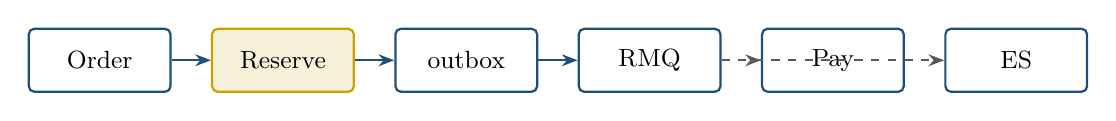
\begin{tikzpicture}[node distance=2mm and 5mm,font=\scriptsize,
    every node/.append style={minimum width=14mm,minimum height=7mm}]
  \node[node-box] (o) {Order};
  \node[node-box,right=of o,node-warn] (rsv) {Reserve};
  \node[node-box,right=of rsv] (ob) {outbox};
  \node[node-box,right=of ob] (mq) {RMQ};
  \node[node-box,right=of mq] (pay) {Pay};
  \node[node-box,right=of pay] (es)  {ES};
  \draw[arrow] (o)   -- (rsv);
  \draw[arrow] (rsv) -- (ob);
  \draw[arrow] (ob)  -- (mq);
  \draw[arrow-async] (mq) -- (pay);
  \draw[arrow-async] (mq) -- (es);
\end{tikzpicture}
\vspace{1mm}
\small 每一步消费上一步事件、产出下一步事件，无总指挥。\\
对 gomall 的 5 步链路是最省心的选择 —— 加新下游 = 新加一个消费者，不改主链路。
\srcnote{docs/blog/04-outbox-saga.md \S 完整链路}
\end{frame}

\begin{frame}{Saga 失败：CancelUnpaidOrder 就是一次补偿}
\begin{tikzpicture}[node distance=10mm and 14mm,font=\scriptsize]
  \node[node-box] (cre)  {1.CreateOrder\\(reserved += n)};
  \node[node-box,right=of cre,node-warn] (wait) {2.等待支付\\(15min 内)};
  \node[node-box,right=of wait,node-bad] (timeout) {3.超时未付};
  \node[node-box,below=of timeout] (cancel) {4.CancelUnpaidOrder};
  \node[node-box,left=of cancel,node-ok] (rel)  {5.Release\\(reserved $\to$ avail)};
  \node[node-box,left=of rel]           (ob)   {6.outbox\\order.cancelled};
  \draw[arrow] (cre) -- (wait);
  \draw[arrow] (wait) -- (timeout);
  \draw[arrow-alert] (timeout) -- (cancel);
  \draw[arrow] (cancel) -- (rel);
  \draw[arrow] (rel) -- (ob);
\end{tikzpicture}
\vspace{2mm}
\small \textbf{业务承诺}：
\begin{itemize}
  \item \textbf{Saga 补偿 $\leq$ 5 min}：超时关单 + 库存回填全链路 5 分钟内闭合。
  \item \textbf{库存不变量}：\texttt{available + reserved + sold = total} 始终成立。
  \item \textbf{先 DB tx 后 cache}：DB 关单 + outbox 一起 commit 后才释放 Redis 占用，失败可重放。
\end{itemize}
\srcnote{service/order\_cancel.go:14--63 完整闭包}
\end{frame}

\begin{frame}{补偿失败的容错：用户感受是什么}
\begin{itemize}
  \item Saga 补偿不是银弹：补偿本身也会失败（cache 拒连 / 网络抖）。
  \item \textbf{gomall 的容错思路}：
  \begin{enumerate}
    \item 先保证 DB commit —— 业务真相先落地（订单确实关了）。
    \item Cache 释放失败只打 error 日志，不回滚 DB —— 状态机靠下次扫描自愈。
    \item 真出现长期不一致时，由 cron + outbox 死信表兜底。
  \end{enumerate}
  \item \textbf{用户感受}：库存可能"短暂少一点"（业务可接受），但绝不"卖超"（业务不可接受）。
  \item \textbf{客服话术}："您的订单已成功取消，库存回填中，最迟 5 分钟可见。"
\end{itemize}
\srcnote{service/order\_cancel.go:55--62 释放 reservation 仅 log，不回滚 DB}
\end{frame}

% ============================================================
\section{缓存一致性：用户多久看到改价}
% ============================================================

\begin{frame}{缓存出错的用户感知}
\begin{tikzpicture}[node distance=8mm and 12mm,font=\scriptsize]
  \node[node-box] (c1) {读 1: cache miss};
  \node[node-box,below=of c1] (w1) {写: 删 cache};
  \node[node-box,right=of w1] (w2) {写: UPDATE DB};
  \node[node-box,right=of c1] (c2) {读 1: 回填旧值 (race)};
  \node[node-box,below=of w2,node-bad] (bad) {cache = 旧值};
  \draw[arrow] (c1) -- (c2);
  \draw[arrow] (w1) -- (w2);
  \draw[arrow] (c2) -- (bad);
  \draw[arrow-bad] (w2) -- (bad);
\end{tikzpicture}
\vspace{2mm}
\textbf{业务出错形态}：
\begin{itemize}
  \item C 端：商品改价后短时间还看到旧价 $\to$ 用户截图投诉"虚假宣传"。
  \item 商家：调完价想"立刻看到生效"$\to$ 自己刷商品页还是旧的 $\to$ 怀疑改价没成功 $\to$ 重复操作。
  \item 运营：促销开始的瞬间，部分用户看到的还是原价 $\to$ 大促转化率统计失真。
\end{itemize}
\srcnote{service/product.go ProductUpdate 写库前后两次 \texttt{DelProductDetail}}
\end{frame}

\begin{frame}{改价生效窗口：三方期望对齐}
\begin{tabular}{@{}lp{2.6cm}p{2.8cm}p{3.0cm}@{}}
\toprule
角色 & 期望窗口 & gomall 实际 & 满足 \\
\midrule
C 端用户  & 改价后 $\leq 5$ 分钟看到新价 & $\leq 1$ s（延迟双删）  & \checkmark 远超期望 \\
商家     & 改价后立刻自己能看到生效     & 写后立即 DEL，自己读必 miss 回源 & \checkmark \\
运营平台  & 全网用户在大促开始秒级同步   & $\leq 1$ s + ES outbox 增量索引 & \checkmark \\
\bottomrule
\end{tabular}
\vspace{2mm}
\small \textbf{业务承诺}：缓存延迟双删 $\leq 1$ s 内全部生效（实测 500 ms 抹掉所有 race）。
\srcnote{repository/cache/product.go:14--17 常量定义}
\end{frame}

\begin{frame}{延迟双删时序图}
\begin{tikzpicture}[node distance=4mm,font=\scriptsize]
  \foreach \name/\x in {Writer/0, Cache/30, DB/60, Reader/90} {
    \node[node-box,minimum width=14mm] at (\x mm,0) (\name) {\name};
    \draw[lifeline] (\x mm,-2mm) -- (\x mm,-50mm);
  }
  \draw[arrow]      (0,-6mm)   -- node[above,font=\tiny]{1.DEL key}      (30mm,-6mm);
  \draw[arrow]      (0,-12mm)  -- node[above,font=\tiny]{2.UPDATE}       (60mm,-12mm);
  \draw[arrow-async](90mm,-18mm)-- node[above,font=\tiny]{并发读到旧值}  (60mm,-18mm);
  \draw[arrow-async](90mm,-24mm)-- node[above,font=\tiny\color{cBad}]{回填旧值}  (30mm,-24mm);
  \draw[arrow,bend right=20](0,-30mm) to node[above,font=\tiny\color{cAccent}]{3.500ms 后再 DEL} (30mm,-30mm);
  \node[font=\tiny] at (45mm,-40mm) {第二次 DEL 抹掉 race 写回的旧值，窗口收敛到亚秒级};
\end{tikzpicture}
\srcnote{repository/cache/product.go:64--74 \texttt{DoubleDeleteAsync}}
\end{frame}

\begin{frame}[fragile]{双删 + 击穿保护：源码}
\begin{lstlisting}[language=Go,firstnumber=55,
  caption={\srcnote{repository/cache/product.go:55--74}}]
// TryProductLock SETNX 抢回源锁，避免缓存击穿时多个请求同时回源
func TryProductLock(ctx context.Context, id uint) (bool, error) {
    return RedisClient.SetNX(ctx, ProductLockKey(id), "1", ProductLockTTL).Result()
}

func UnlockProduct(ctx context.Context, id uint) {
    RedisClient.Del(ctx, ProductLockKey(id))
}

// DoubleDeleteAsync 延迟双删：写库后已经做了第一次删除，这里在 interval 后再删一次，
// 用于覆盖"读旧值的并发请求把旧值塞回缓存"的窗口。
func DoubleDeleteAsync(id uint, interval time.Duration) {
    if interval <= 0 { interval = ProductDelayInterval }  // 默认 500ms
    go func() {
        time.Sleep(interval)
        _ = RedisClient.Del(context.Background(), ProductDetailKey(id)).Err()
    }()
}
\end{lstlisting}
\vspace{1mm}
\small \textbf{业务读法}：\texttt{SetNX} 单进程拿回源锁；\texttt{ProductLockTTL=3s} 防死锁；\texttt{goroutine} 不阻塞写接口（商家点保存即时返回）；\texttt{context.Background()} 因为商家请求已返回但 500 ms 后还要补一刀。
\end{frame}

\begin{frame}{击穿保护：SETNX 单飞回源}
\begin{tikzpicture}[node distance=8mm and 10mm,font=\scriptsize]
  \node[node-box] (r1) {读 A};
  \node[node-box,right=of r1] (r2) {读 B};
  \node[node-box,right=of r2] (r3) {读 C};
  \node[node-box,below=of r2,node-warn] (lock) {SETNX lock\\TTL 3s};
  \node[node-box,below=of lock] (db) {DB SELECT};
  \node[node-box,right=of db,node-ok] (set) {SET cache};
  \draw[arrow] (r1) -- (lock);
  \draw[arrow-bad,bend left=15] (r2) to node[above,font=\tiny]{抢锁失败 / 退避} (r1.east);
  \draw[arrow-bad,bend right=15] (r3) to node[above,font=\tiny]{抢锁失败 / 退避} (r1.east);
  \draw[arrow] (lock) -- (db);
  \draw[arrow] (db) -- (set);
\end{tikzpicture}
\vspace{2mm}
\small \textbf{业务收益}：首页 banner 商品 cache 失效瞬间不会让 1000 个请求一起打到 DB；落库次数从 $N$ 降到 1 + 其余复用 cache。\\
\textbf{用户感受}：首页商品永远秒开，永远不会"突然变慢 5 秒"。
\srcnote{repository/cache/product.go:55--62 \texttt{TryProductLock} / \texttt{UnlockProduct}}
\end{frame}

% ============================================================
\section{业务码与压测：用数字背书}
% ============================================================

\begin{frame}{业务码全表对照}
\begin{tabular}{@{}lll@{}}
\toprule
业务码 & 含义 & 与一致性的关联 \\
\midrule
\textbf{60002} & 重复请求处理中 & 幂等 Lua 状态机，下游消费 outbox 必须返这个 \\
\textbf{50001} & OSS / 库存等下游异常 & 缓存击穿 / 回源失败 / Saga 补偿入口 \\
\textbf{70001} & 限流 & 客户端重试触发 = 重复事件 = 必须幂等 \\
\textbf{70002} & 熔断 & 下游 dead 时上游主动断 \\
30001/30002/30005 & 鉴权三类失败 & 客服优先排除身份问题 \\
20001 & boss token & 商家自助 API 鉴权（路线图） \\
\bottomrule
\end{tabular}
\vspace{2mm}
\small 所有业务码全表见 \texttt{pkg/e/code.go}，客服话术配套见 README 业务全景表。
\srcnote{pkg/e/code.go 业务码全表}
\end{frame}

\begin{frame}{压测里量出来的两组真实数字}
\begin{tabular}{@{}lr@{}}
\toprule
压测场景 & 实测 \\
\midrule
单元测试 \texttt{TestCoupon\_AtomicClaimNoOversell}：500 并发抢 100 张券 & \textbf{零超发} \\
压测 \texttt{idempotency\_replay.js}：同 Key 累计 15s 请求    & \textbf{755{,}033} \\
\hspace{4mm}对应入库订单数（\texttt{SELECT COUNT(*)}）          & \textbf{1} \\
\hspace{4mm}回放 p95 / 吞吐                                    & 2.33 ms / \textbf{50{,}319 RPS} \\
\hspace{4mm}基线 \texttt{/ping}                               & 3.51 ms / 64{,}254 RPS \\
\bottomrule
\end{tabular}
\vspace{3mm}
\small "零超发" + "75 万次只入 1 单" 是同一套设计的两个表现 ——
\textbf{at-least-once 投递}遇上\textbf{业务码幂等键}（券号 / Idempotency-Key），
最终对账数永远只算一次。
\srcnote{stressTest/REPORT.md \S 各链路压测结果 / \S 4. 幂等中间件压测}
\end{frame}

\begin{frame}{Outbox 解决"丢失"，幂等解决"重复"}
\begin{tikzpicture}[node distance=8mm and 12mm,font=\scriptsize]
  \node[node-box] (a) {应用};
  \node[node-box,right=of a] (db)  {DB + outbox};
  \node[node-box,right=of db,node-warn] (mq) {RMQ};
  \node[node-box,right=of mq,node-ok] (idem) {幂等表 / Key};
  \node[node-box,right=of idem] (down) {下游 handler};
  \draw[arrow] (a) -- (db);
  \draw[arrow] (db) -- (mq);
  \draw[arrow-async] (mq) -- (idem);
  \draw[arrow] (idem) -- (down);
  \draw[arrow,bend right=25] (mq.south) to
       node[below,font=\tiny\color{cWarn}]{重复投递 (网络 / publisher 重启)} (idem.south);
\end{tikzpicture}
\vspace{2mm}
\small 投递语义：\textbf{at-least-once} —— 至少一次。\\
\textbf{at-least-once + 业务幂等键} = 业务侧 exactly-once。
\srcnote{deck 01 幂等中间件 / deck 04 outbox / deck 05 限流熔断 三者衔接}
\end{frame}

% ============================================================
\section{真实事故复盘：用户怎么感知到的}
% ============================================================

\begin{frame}{事故一：未支付订单取消导致虚高库存}
\textbf{用户感知}（commit 5c9ae27 前）：商品页"库存 999"$\to$ 真去下单"库存不足"$\to$ 一头雾水。

\vspace{2mm}
\textbf{根因链}：
\begin{enumerate}
  \item 旧版 \texttt{CancelUnpaidOrder} 把 \texttt{product.num} 加回 DB —— 但未支付订单\textbf{从未真正扣减过} DB 库存（只占了 Redis reserved）。
  \item 第一次取消：DB.num \texttt{+= n}；Redis.reserved \texttt{-= n} —— 库存虚高 n。
  \item 累计 100 个超时订单 = 库存虚高 100 倍。
\end{enumerate}
\vspace{1mm}
\textbf{修复}（PR \#58 引入预扣 + Saga）：
\begin{itemize}
  \item DB.num 只在\textbf{支付成功}时递减，未支付订单只动 Redis reserved。
  \item CancelUnpaidOrder \textbf{不再}写 \texttt{product.num}，只释放 Redis reserved。
  \item 库存不变量：\texttt{available + reserved + sold = total} 始终成立。
\end{itemize}
\srcnote{service/order\_cancel.go:14--18 注释 "不再回写 product.Num"}
\end{frame}

\begin{frame}{事故二：搜索索引腐烂 12 小时无人知}
\textbf{用户感知}（commit a43cf61 前）：商品改价后，搜索结果一直显示旧价；商详页正常。用户点进去发现价格不一样 $\to$ 投诉"虚假宣传"。

\vspace{2mm}
\textbf{根因链}：
\begin{enumerate}
  \item 旧链路：商品 UPDATE 时\textbf{同步}调用 ES 重建索引。
  \item ES 集群偶发拒连 $\to$ 同步调用失败 $\to$ 业务 \texttt{rollback} $\to$ 商家投诉"我改不了价"。
  \item 业务为了不影响下单，把 ES 写入改成\textbf{忽略错误}。
  \item ES 失败被吞，索引与 DB 漂移 12 小时无人知。
\end{enumerate}
\vspace{1mm}
\textbf{修复}（PR \#59 切到 outbox + 消费者）：
\begin{itemize}
  \item 商品 UPDATE 同事务\textbf{只写 outbox\_event}，不直接写 ES。
  \item ES 消费者从 RMQ 拉事件，失败有重试 + 死信。
  \item 死信触发 alarm，值班 5 分钟内看到（SRE SOP）。
\end{itemize}
\srcnote{commit a43cf61 商品搜索切换到 ES 通过 outbox + 消费者保持增量索引}
\end{frame}

\begin{frame}{事故三：InitLog 顺序错让全站 503}
\textbf{用户感知}：RabbitMQ 服务下线维护时，gomall 进程\textbf{整体退出}，HTTP 接口全 503 $\to$ \textbf{GMV 归零}。

\vspace{2mm}
\textbf{根因链}（branch \texttt{fix/init-log-order-before-rmq}）：
\begin{enumerate}
  \item \texttt{tryInitRabbitMQ()} 的 \texttt{recover} 块里调用 \texttt{LogrusObj.Warnf}。
  \item 当时 \texttt{util.InitLog()} 反而在它\textbf{之后}。
  \item \texttt{LogrusObj == nil} $\to$ recover 内再次 panic $\to$ 进程退出。
  \item RMQ \textbf{应该}是可选依赖（延迟关单可降级），实际把整个进程拖死。
\end{enumerate}
\vspace{1mm}
\textbf{业务影响}：服务起不来 = 全站瘫痪 = GMV 归零 = P0 事故。
\srcnote{cmd/main.go:30--31 修复后的顺序；stressTest/REPORT.md \S 已修：\texttt{util.LogrusObj}}
\end{frame}

\begin{frame}{修复后的启动顺序（业务因果）}
\begin{tikzpicture}[node distance=5mm and 6mm,font=\scriptsize,
    every node/.append style={minimum width=22mm,minimum height=7mm}]
  \node[node-box] (cfg)  {1.InitConfig};
  \node[node-box,right=of cfg,node-warn] (log) {2.InitLog\\(必须在 recover 之前)};
  \node[node-box,right=of log] (db)   {3.InitMySQL};
  \node[node-box,below=of cfg] (cache){4.InitCache};
  \node[node-box,right=of cache] (sf) {5.Snowflake};
  \node[node-box,right=of sf] (cron)  {6.InitCron};
  \node[node-box,below=of cache] (inv){7.InitInventory};
  \node[node-box,right=of inv] (rmq)  {8.tryInitRabbitMQ};
  \node[node-box,right=of rmq] (pub)  {9.InitOutboxPublisher};
  \draw[arrow] (cfg) -- (log);
  \draw[arrow] (log) -- (db);
  \draw[arrow] (db) -- (cache);
  \draw[arrow] (cache) -- (sf);
  \draw[arrow] (sf) -- (cron);
  \draw[arrow] (cron) -- (inv);
  \draw[arrow] (inv) -- (rmq);
  \draw[arrow] (rmq) -- (pub);
\end{tikzpicture}
\vspace{2mm}
\small 关键约束：\textbf{InitLog 必须在 InitMySQL / RMQ 之前}，因为后续所有 \texttt{tryInit*} 的 \texttt{recover} 都依赖 \texttt{LogrusObj}。
\srcnote{cmd/main.go:29--47 完整初始化序列}
\end{frame}

\begin{frame}{两条可复用的业务侧教训}
\begin{enumerate}
  \item \textbf{初始化顺序}：所有依赖全局对象的代码，必须在它初始化之后才能调用。
  \begin{itemize}
    \item \texttt{InitLog} / \texttt{InitTracer} / \texttt{InitMetrics} 放最前。
    \item 业务承诺：所有外部依赖独立 \texttt{tryInit*} 包装 + recover，主链路（下单/支付/列表/详情）永远在线。
  \end{itemize}
  \item \textbf{recover 内禁止再 panic}：
  \begin{itemize}
    \item recover 是最后兜底，里面再崩进程彻底失控。
    \item 写法：recover 内只 \texttt{fmt.Fprintln(os.Stderr, ...)} 或写本地文件，不依赖任何复杂组件。
  \end{itemize}
\end{enumerate}
\keypoint{outbox publisher 起不来不算事故 —— 启动顺序错了让全站 503，才是事故。}
\srcnote{cmd/main.go:54--62 \texttt{tryInitRabbitMQ} 的 recover 块}
\end{frame}

% ============================================================
\section{业务承诺与边界}
% ============================================================

\begin{frame}{三档一致性窗口：写在 SLO 里}
\begin{tabular}{@{}lp{2.6cm}p{4.4cm}p{3.0cm}@{}}
\toprule
档位 & 窗口上限 & 业务场景 & gomall 落点 \\
\midrule
强一致         & 100 ms 内      & 同一事务可见性、行锁内的预扣 & 库存预扣 (Redis Lua) \\
近实时一致     & 1 s 内         & 用户感知"操作完成 = 立刻可见" & Outbox publish + ES 索引 \\
最终一致       & 5 min 内       & 跨服务对账、数仓同步         & 死信复盘、cron 巡检 \\
\bottomrule
\end{tabular}
\vspace{2mm}
\small \textbf{对外业务承诺}：
\begin{itemize}
  \item 用户下单后 \textbf{$\leq 1$ s} 在订单列表看到（近实时档）。
  \item 商品改价后 \textbf{$\leq 1$ s} 商品详情显示新价（双删窗口）。
  \item 库存与订单的对账差异 \textbf{$\leq 5$ min} 闭合（夜间 cron）。
  \item Outbox sent rate \textbf{$\geq 99.99\%$}（每万条事件最多 1 条进 dead）。
  \item Saga 补偿 \textbf{$\leq 5$ min} 全链路闭合。
\end{itemize}
\srcnote{README.md \S 业务承诺（SLO）；service/outbox/publisher.go:23 PollInterval=1s}
\end{frame}

\begin{frame}{业务边界：本一致性方案不做什么}
诚实列出（参考 README \S 业务边界）：
\begin{itemize}
  \item \textbf{不用 2PC / XA}：协调者持锁拖死 p99，业务 RT 不可接受；MySQL 之外的存储都不支持 XA。
  \item \textbf{不用 TCC}：每个接口要写 Try / Confirm / Cancel 三份，业务侵入太重；gomall 用 outbox 异步事件做等价语义。
  \item \textbf{不用 binlog CDC}（Canal / Debezium）：表数量 $\approx 12$、消费者全 Go、单 publisher 没瓶颈，引入 CDC ROI 不正。
  \item \textbf{不做事件溯源全量重放}：outbox 表只追加（无 Delete 路径），为未来演进留门，但目前不维护快照 / 投影。
  \item \textbf{不做跨地域多活同步}：单机房部署，多活留给规模到达后再上。
  \item \textbf{不做 RocketMQ 事务消息}：gomall 用 RabbitMQ，事务消息是 RocketMQ 专属能力。
\end{itemize}
\srcnote{README.md \S 业务边界；docs/blog/04-outbox-saga.md \S 为什么不用 2PC}
\end{frame}

\begin{frame}{业务侧总结：一致性约束一张表}
\begin{tabular}{@{}llll@{}}
\toprule
一致性对 & 模式 & 业务码 / 表 & gomall 现状 \\
\midrule
DB $\leftrightarrow$ MQ      & Transactional Outbox  & \texttt{outbox\_event.status} & pending/sent/dead \\
DB $\leftrightarrow$ Cache   & Cache Aside + 延迟双删 & \texttt{product:detail:\{id\}} & 500 ms 双删 \\
缓存击穿                     & SETNX 单飞回源        & \texttt{product:lock:\{id\}}   & TTL 3 s \\
跨服务 Saga                  & 协同式 (事件驱动)     & 见 outbox 路由 key            & 5 步链路 \\
启动依赖                     & 顺序约束             & N/A                            & InitLog 第 2 位 \\
\bottomrule
\end{tabular}
\vspace{2mm}
\small 五对一致性各有客诉链路、各有兜底、各有业务承诺；缺一不可。
\srcnote{cmd/main.go / repository/cache/product.go / repository/db/dao/outbox.go}
\end{frame}

% ============================================================
\appendix
% ============================================================

\begin{frame}{面试 Q\&A（1/3）}
\textbf{Q1}：为什么 Outbox 比"DB commit 后再 publish"安全？\\
\hspace{4mm}\small A：commit 与 publish 不在一个事务，commit 成功 publish 失败就丢事件 $\to$ 商家收不到发货事件、库存不回。Outbox 把事件写进 DB，由轮询消化，事件丢失等价于 DB 数据丢失。\srcnote{service/order\_cancel.go:31--51}

\vspace{2mm}
\textbf{Q2}：outbox 表会不会堆积？\\
\hspace{4mm}\small A：会。监控 \texttt{status=pending AND next\_retry\_at <= now()} 的行数即可。横向扩展用 \texttt{SELECT FOR UPDATE SKIP LOCKED}；当前 gomall 单实例 BatchSize=100/1s 还远没到瓶颈。\srcnote{repository/db/dao/outbox.go:43--51}

\vspace{2mm}
\textbf{Q3}：延迟双删的"延迟"该取多大？\\
\hspace{4mm}\small A：取\textbf{大于}最长读 race 窗口。gomall 取 500ms：DB 写常态 5--20ms，留 20$\times$ 余量盖 GC / 网络抖动；TTL 10min 兜底。\srcnote{repository/cache/product.go:14--17}

\vspace{2mm}
\textbf{Q4}：协同式 vs 编排式 Saga，怎么选？\\
\hspace{4mm}\small A：步骤 $\leq 5$、跨团队少 $\to$ 协同（gomall 选）。步骤多、需可视化看板、跨团队多 $\to$ 编排，但要承担"中心节点"运维成本。\srcnote{docs/blog/04-outbox-saga.md \S 完整链路}
\end{frame}

\begin{frame}{面试 Q\&A（2/3）}
\textbf{Q5}：为什么 cache 释放失败不回滚 DB？\\
\hspace{4mm}\small A：DB 是业务真相，cache 是性能侧。Cache 失败让库存"短暂少一点"，最坏拒单不超卖；回滚 DB 反而让"已关单"被复活，业务码乱套，客服更难解释。\srcnote{service/order\_cancel.go:55--62}

\vspace{2mm}
\textbf{Q6}：客服来问"用户的退款 24h 没回来"怎么查？\\
\hspace{4mm}\small A：\texttt{SELECT status, attempts, last\_error FROM outbox\_event WHERE aggregate\_type='order' AND aggregate\_id=? ORDER BY id}。status=1 排队中 / 2 已发下游 / 3 dead 需升 SRE。\srcnote{repository/db/model/outbox.go:24--35}

\vspace{2mm}
\textbf{Q7}：2PC / XA 为什么不用？\\
\hspace{4mm}\small A：协调者单点 + 同步阻塞 + 异构资源不支持（Redis/RMQ/ES 都没 XA）。业务 RT 不可接受（下单 p99 从 5ms 拉到 100ms+，违反 SLO）。\srcnote{docs/blog/04-outbox-saga.md \S 为什么不用 2PC}

\vspace{2mm}
\textbf{Q8}：业务承诺的"1 秒可见"怎么保证？\\
\hspace{4mm}\small A：PollInterval=1s + BatchSize=100 + 单实例 $< 100$ ev/s 峰值 $\to$ 平均延迟 $< 500$ ms，最坏 1s。监控 \texttt{outbox\_publish\_latency\_p99 > 1s} 报警。\srcnote{service/outbox/publisher.go:21--32}
\end{frame}

\begin{frame}{面试 Q\&A（3/3）}
\textbf{Q9}：MaxAttempts=10 怎么算出来的？退避 5min 封顶又是为什么？\\
\hspace{4mm}\small A：1+2+4+8+16+32+64+128+256+300=811s$\approx$13.5min 累计窗口，覆盖一次"中等故障"够用；封顶 5min 防止退避无限拉长导致积压堆 outbox 表。\srcnote{repository/db/dao/outbox.go:62--78}

\vspace{2mm}
\textbf{Q10}：进 dead 的事件谁来处理？\\
\hspace{4mm}\small A：触发报警 $\to$ 值班 SRE 看 \texttt{last\_error} $\to$ 联系下游确认修复 $\to$ SQL 改回 \texttt{status=1, attempts=0, next\_retry\_at=now()} $\to$ publisher 自动重发。\textbf{绝不}自动改回 pending。\srcnote{repository/db/dao/outbox.go:69--70}

\vspace{2mm}
\textbf{Q11}：为什么 \texttt{drainBatch} 第一行要判 \texttt{rabbitmq.GlobalRabbitMQ == nil}？\\
\hspace{4mm}\small A：静默降级。RMQ 未起时 publisher 不发事件、不动 DB；主链路（下单 / 支付）继续在线，事件堆 outbox 等 RMQ 恢复后自动消化。\srcnote{service/outbox/publisher.go:66--68}

\vspace{2mm}
\textbf{Q12}：业务侧怎么承诺"最终一致"的窗口？\\
\hspace{4mm}\small A：分三档：库存预扣 100ms、订单/搜索可见 1s、跨服务对账 5min。对外 SLO 写明上限，超过触发 P2 报警；客服话术按这三档给用户解释。\srcnote{service/outbox/publisher.go:21--32 与 README SLO 表}
\end{frame}

\begin{frame}{代码位置一览}
\begin{description}
  \item[outbox\_event 表]\srcnote{repository/db/model/outbox.go:9--37}
  \item[Outbox DAO (Insert / FetchBatch / MarkSent / MarkFailed)]\srcnote{repository/db/dao/outbox.go:13--86}
  \item[Publisher (Start / loop / drainBatch)]\srcnote{service/outbox/publisher.go:34--86}
  \item[初始化 publisher]\srcnote{initialize/outbox.go (InitOutboxPublisher)}
  \item[OrderCreate (业务 + outbox 同事务)]\srcnote{service/order.go::CreateOrder}
  \item[CancelUnpaidOrder (Saga 补偿)]\srcnote{service/order\_cancel.go:14--63}
  \item[缓存双删 / SETNX 回源锁]\srcnote{repository/cache/product.go:13--74}
  \item[ProductUpdate 调用双删]\srcnote{service/product.go ProductUpdate}
  \item[启动顺序修复点]\srcnote{cmd/main.go:29--47；branch fix/init-log-order-before-rmq}
  \item[业务码全表]\srcnote{pkg/e/code.go}
  \item[压测数据源]\srcnote{stressTest/REPORT.md}
\end{description}
\keypoint{配套：deck 04-cart-to-order / deck 07-inventory / deck 09-order-lifecycle / docs/blog/04-outbox-saga.md}
\end{frame}

\end{document}
